\documentclass[11pt,a4paper]{article}
\usepackage[utf8]{inputenc}
\usepackage[T1]{fontenc}
\usepackage{amsmath,amssymb,amsfonts,bm}
\usepackage{geometry}
\geometry{a4paper, margin=18mm, top=20mm, bottom=22mm}
\usepackage{graphicx}
\usepackage{booktabs}
\usepackage{array}
\usepackage{listings}
\usepackage{xcolor}
\usepackage{titlesec}
\usepackage{fancyhdr}
\usepackage{hyperref}
\usepackage{microtype}
\usepackage{enumitem}

% Palette
\definecolor{siestaBlue}{RGB}{30, 64, 175}
\definecolor{siestaNavy}{RGB}{15, 23, 42}
\definecolor{siestaCyan}{RGB}{2, 132, 199}
\definecolor{siestaGreen}{RGB}{16, 185, 129}
\definecolor{siestaAmber}{RGB}{217, 119, 6}
\definecolor{codeBg}{RGB}{248, 250, 252}
\definecolor{codeBorder}{RGB}{203, 213, 225}

\hypersetup{
 colorlinks=true,
 linkcolor=siestaBlue,
 filecolor=siestaCyan, 
 urlcolor=siestaBlue,
 citecolor=siestaGreen,
 pdftitle={SIESTA Input Builder: Comprehensive User Manual & Hidden Features Handbook},
    pdfauthor={SIESTA Materials Science DFT Initiative},
 pdfsubject={Detailed Step-by-Step Operations, Hidden Features, and Workflow Guide for SIESTA Input Builder GUI},
 pdfkeywords={SIESTA, GUI, FDF, VASP, ASE GUI, Constraints, CI-NEB, Phonons, Work Function, Band Alignment}
}

\titleformat{\section}
 {\normalfont\Large\bfseries\color{siestaNavy}}{\thesection}{1em}{}[\titlerule]
\titleformat{\subsection}
 {\normalfont\large\bfseries\color{siestaBlue}}{\thesubsection}{1em}{}
\titleformat{\subsubsection}
 {\normalfont\normalsize\bfseries\color{siestaCyan}}{\thesubsubsection}{1em}{}

\lstset{
 backgroundcolor=\color{codeBg},
 basicstyle=\ttfamily\footnotesize,
 breaklines=true,
 frame=single,
 rulecolor=\color{codeBorder},
 numbers=none,
 keywordstyle=\color{siestaBlue}\bfseries,
 commentstyle=\color{gray}\itshape,
 stringstyle=\color{siestaAmber},
 keepspaces=true,
 showstringspaces=false,
 tabsize=2,
 xleftmargin=2mm,
 xrightmargin=2mm
}

\pagestyle{fancy}
\fancyhf{}
\fancyhead[L]{\small\color{gray}\textit{SIESTA Input Builder: Complete GUI Manual \& Hidden Features}}
\fancyhead[R]{\small\color{siestaBlue}\textbf{Web Studio Operations Guide}}
\fancyfoot[C]{\thepage}
\renewcommand{\headrulewidth}{0.4pt}
\renewcommand{\footrulewidth}{0.4pt}

\title{\Huge \textbf{SIESTA Input Builder Web Studio}\\[0.3em]
\Large \textbf{The Complete GUI User Manual \& Hidden Features Handbook}\\[0.4em]
\large \textit{A Comprehensive, Step-by-Step Operational Reference Covering Every Button, Section, Converter, Analysis Suite, and Power-User Workflow}}
\author{\textbf{SIESTA Open-Source Development Consortium}\\
\small Computational Materials Science \& Surface Physics Initiative}
\date{\textbf{October 2026} \quad | \quad \textbf{App Version 5.4.2 (Production)}}

\begin{document}
\maketitle

\begin{abstract}
\noindent The \textbf{SIESTA Input Builder} is an open-source, client-side web application designed to eliminate the steep learning curve, manual formatting errors, and scattered keyword documentation of the SIESTA density functional theory (DFT) software suite. Providing an intuitive graphical interface equivalent to BURAI or pw.gui for Quantum ESPRESSO, it covers the complete operational lifecycle: from initial crystal import (CIF/POSCAR) to advanced constraints, reaction path CI-NEB interpolation, vibrational phonon matrices, real-space surface work functions, and execution time accounting. This handbook serves as the exhaustive operational reference, detailing every screen, button, drawer, and hidden shortcut across the 13 modular sections.
\end{abstract}

\tableofcontents
\newpage

% ── SECTION 1 ───────────────────────────────────────────────────────────────
\section{Application Architecture \& Global Workflow}

\subsection{Zero-Backend Security \& Privacy Architecture}
Unlike cloud DFT portals that require uploading sensitive structure files to third-party remote servers, the SIESTA Input Builder runs \textbf{100\% inside your local browser}:
\begin{itemize}[leftmargin=*]
 \item \textbf{No Server Computing:} Built with React 19, Vite, and Zustand. All CIF parsing, VASP coordinate transformations, 3D WebGL rendering, and FDF generation take place in your browser's V8 JavaScript engine.
 \item \textbf{Confidentiality of Novel Materials:} Proprietary atomic coordinates, unreleased battery/catalyst crystal structures, and unpublished coordinates never cross the network. You can disconnect your internet entirely after opening the site, and the application remains fully functional.
 \item \textbf{Zero Installation Friction:} Requires no Python environments, no compilation of GUI toolkits (Tkinter/Qt), and no local server daemons. Works across Linux, macOS, Windows, and tablet browsers.
\end{itemize}

\subsection{The Three-Panel Layout}
The application interface is divided into three functional areas:
\begin{enumerate}[leftmargin=*]
 \item \textbf{Top Toolbar (Header):} Global project controls, one-click template presets, convergence sweep package generators, CIF/FDF import, validation engine, export actions, and Dark/Light theme switching.
 \item \textbf{Left Navigation Sidebar:} The master index providing rapid switching between all 13 specialized calculation sections, accompanied by a dynamic real-time validation warning badge.
 \item \textbf{Main Workspace Pane:} The active form interface with contextual tooltips, parameter units, interactive data grids, 3D visualizers, and analysis studios.
 \item \textbf{Right-Hand Live FDF Preview Pane:} A persistent 320px wide code drawer that regenerates the exact, formatted, production-ready \texttt{.fdf} file on every single keystroke.
\end{enumerate}

\begin{figure}[h!]
\centering
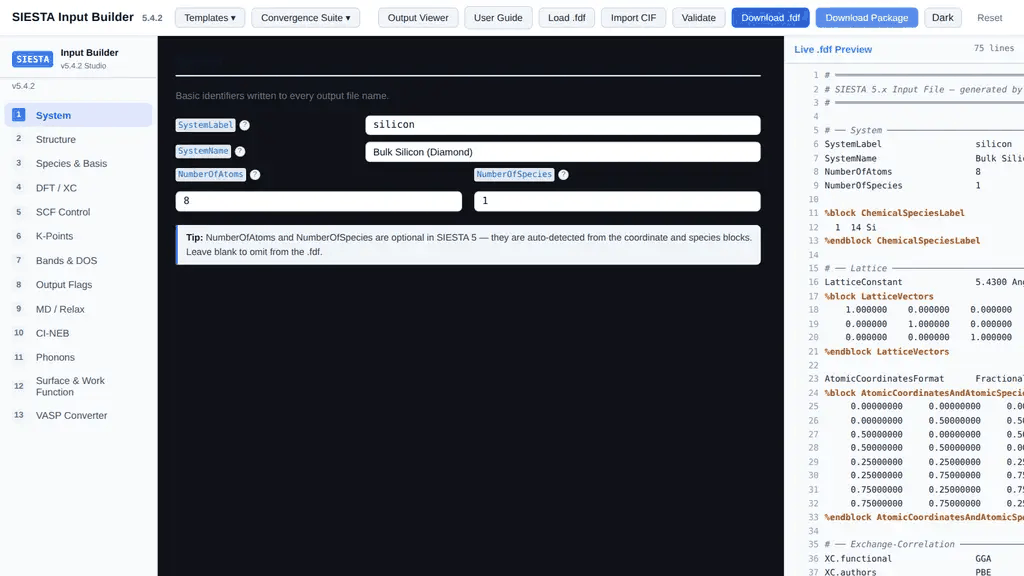
\includegraphics[width=0.92\textwidth]{figures/fig01_overview.png}
\caption{SIESTA Input Builder user interface showing Top Toolbar, 13-section Sidebar navigation, Section 1 System inputs, and persistent Live FDF Preview pane.}
\end{figure}


\subsection{Dark and Light Mode Switching}
Located in the upper right of the Toolbar:
\begin{itemize}[leftmargin=*]
 \item \textbf{\texttt{Dark} Mode (Default):} Tailored for long computing sessions and night research. High-contrast slate backgrounds (\texttt{\#0f1117}) with vibrant syntax accents.
 \item \textbf{\texttt{Light} Mode:} Crisp, publication-white canvas (\texttt{\#ffffff}) with deep slate typography (\texttt{\#0f172a}). Ideal for capturing clean figures, creating presentation slides, and working in bright daylight.
 \item \textbf{State Persistence:} The selected theme is stored in browser \texttt{localStorage} under \texttt{siesta\_theme}, restoring your preferred appearance across browser refreshes.
\end{itemize}

\newpage
% ── SECTION 2 ───────────────────────────────────────────────────────────────
\section{The Global Toolbar \& Top Navigation}

\subsection{Pre-Configured Calculation Templates (\texttt{Templates ▾})}
The \textbf{Templates} dropdown allows instant population of standard scientific workflows in a single click:
\begin{itemize}[leftmargin=*]
 \item \textbf{Bulk SCF (Single-Point):} Sets up high-precision total energy calculation on periodic crystals. Configures \texttt{MaxSCFIterations 100}, \texttt{DM.Tolerance 1.0d-4}, \texttt{MeshCutoff 300 Ry}, and Monkhorst-Pack $k$-grid.
 \item \textbf{Geometry Relaxation (CG):} Configures atomic position minimization via Conjugate Gradient (\texttt{MD.TypeOfRun CG}), sets force tolerance to \texttt{0.04 eV/\AA}, and requests force output (\texttt{WriteForces true}).
 \item \textbf{Variable-Cell Relaxation:} Optimizes both atomic positions and cell vectors (\texttt{MD.VariableCell true}), maintaining stress tolerance at \texttt{1.0 GPa}.
 \item \textbf{Band Structure Calculation:} Configures SCF convergence followed by dispersion tracking along high-symmetry $k$-lines (\texttt{BandLinesScale ReciprocalLatticeVectors}).
 \item \textbf{Slab / Surface Calculation:} Automatically expands unit cell along $z$, enables \texttt{Slab.DipoleCorrection true}, enforces $k_z = 1$, and requests electrostatic potential output (\texttt{SaveElectrostaticPotential true}).
 \item \textbf{Density of States (DOS + PDOS):} Configures orbital-resolved projected DOS energy window (\texttt{EF -10.0 10.0 0.1 1000 eV}) and dense $k$-mesh.
\end{itemize}

\subsection{Automated Convergence Suite Generator (\texttt{Convergence Suite ▾})}
Achieving publication-grade DFT results requires proving that your energy and lattice parameters are converged with respect to numerical cutoffs. The toolbar provides automated zip package generators:
\begin{enumerate}[leftmargin=*]
 \item \textbf{MeshCutoff Sweep (\texttt{MeshCutoff Sweep (.zip)}):}
 \begin{itemize}
 \item Generates a complete series of individual FDF files stepping from 150 Ry to 500 Ry (150, 200, 250, 300, 350, 400, 450, 500 Ry).
 \item Includes an automated parallel bash runner script (\texttt{run\_mesh.sh}) with SLURM/MPI execution commands.
 \item Includes a Python script (\texttt{plot\_mesh\_convergence.py}) using \texttt{matplotlib} to extract total energies from stdout and plot the convergence plateau ($|\Delta E| < 1\text{ meV/atom}$).
 \end{itemize}
 \item \textbf{K-Grid Sweep (\texttt{K-Grid Sweep (.zip)}):}
 \begin{itemize}
 \item Generates a series of $k$-mesh densities ($4\times4\times4, 6\times6\times6, 8\times8\times8, 10\times10\times10, 12\times12\times12$).
 \item Automatically respects 2D slab geometry if active ($N_x \times N_y \times 1$).
 \item Bundles automated runner and convergence plotting scripts.
 \end{itemize}
\end{enumerate}

\subsection{File Import Engines: CIF and FDF}
\begin{itemize}[leftmargin=*]
 \item \textbf{\texttt{Import CIF}:} Ingests raw \texttt{.cif} files from databases (Materials Project, ICSD, COD, AFLOW, VESTA). The client-side CIF parser extracts:
 \begin{itemize}
 \item Lattice parameters ($a, b, c, \alpha, \beta, \gamma$) and converts them to Cartesian lattice vectors.
 \item Atomic coordinates and fractional space-group symmetry expansions.
 \item Chemical element symbols and automatically assigns atomic numbers $Z$.
 \item Populates Section 1, 2, and 3 simultaneously.
 \end{itemize}
 \item \textbf{\texttt{Load .fdf}:} Round-trip loader. Ingests any legacy or modern SIESTA input file, parses keywords and blocks, and repopulates every form control across all sections.
\end{itemize}

\subsection{Interactive Validation Engine (\texttt{Validate})}
Clicking **Validate** runs a comprehensive consistency check against official SIESTA rules:
\begin{itemize}[leftmargin=*]
 \item Flags empty or invalid \texttt{SystemLabel} identifiers.
 \item Verifies that species indices in \texttt{AtomicCoordinatesAndAtomicSpecies} match entries in \texttt{ChemicalSpeciesLabel}.
 \item Warns if \texttt{MD.VariableCell true} is active on a surface slab with unconstrained $c$-axis.
 \item Flags non-physical cutoffs (e.g., \texttt{MeshCutoff < 100 Ry}).
 \item Highlights errors with a red badge in the sidebar and lists exact remedy steps.
\end{itemize}

\subsection{Export Mechanisms: Plain FDF vs. Complete Cluster Package}
\begin{itemize}[leftmargin=*]
 \item \textbf{\texttt{Download .fdf}:} Downloads the single active \texttt{.fdf} input file.
 \item \textbf{\texttt{Download Package}:} The recommended export for HPC clusters. Downloads a ready-to-run \texttt{.zip} package containing:
 \begin{enumerate}
 \item \texttt{SystemLabel.fdf}: The complete calculation input.
 \item \texttt{run\_siesta.sh}: Production bash submission script configured with your specified pseudopotential directory:
\begin{lstlisting}[language=bash]
#!/bin/bash
# Auto-generated by SIESTA Input Builder
export SIESTA_PS_PATH="/scratch/user/pseudos"
export SIESTA_PP_PATH="/scratch/user/pseudos"
mpirun -np 4 siesta < SystemLabel.fdf | tee SystemLabel.out
\end{lstlisting}
 \item \texttt{README\_RUN.txt}: Execution instructions, MPI core recommendations, and post-processing commands.
 \end{enumerate}
\end{itemize}

\newpage
% ── SECTION 3 ───────────────────────────────────────────────────────────────
\section{Section-by-Section Walkthrough \& Hidden Details}

\subsection{Section 1 System: Basic Identifiers \& Auto-Detection}
\begin{itemize}[leftmargin=*]
 \item \textbf{\texttt{SystemLabel}:} The core naming string prefixed to all calculation output files (e.g. \texttt{SystemLabel.out}, \texttt{.DM}, \texttt{.bands}, \texttt{.ANI}, \texttt{.VH}, \texttt{.times}). Avoid spaces or special characters.
 \item \textbf{\texttt{SystemName}:} A descriptive title for human readability.
 \item \textbf{Hidden Power Detail (SIESTA 5 Auto-Detection):} In legacy SIESTA 4.x, \texttt{NumberOfAtoms} and \texttt{NumberOfSpecies} were mandatory. In modern SIESTA 5.x, these values are automatically counted by the code from the coordinate and species blocks. If you leave these fields blank in the GUI, the builder cleanly omits them from the FDF, preventing count mismatch errors when adding or removing atoms!
\end{itemize}

\subsection{Section 2 Structure: Lattice, Slabs \& 3D Crystal Viewer}

\subsubsection{Coordinate Formats and Units}
The \texttt{AtomicCoordinatesFormat} selector toggles how atomic positions are interpreted:
\begin{itemize}[leftmargin=*]
 \item \texttt{Fractional}: Dimensionless values $0.0 \le u, v, w < 1.0$ relative to unit cell basis vectors.
 \item \texttt{NotScaledCartesianAng}: Direct Cartesian positions $(x, y, z)$ in \AA ngstr{\"o}ms.
\end{itemize}

\subsubsection{Slab Cleavage \& Vacuum Engineering}
Located in the dedicated ** Slab \& Vacuum Tools** card:
\begin{itemize}[leftmargin=*]
 \item \textbf{Add Vacuum Along Z:} Specify desired vacuum thickness (e.g. \texttt{15.0 \AA} or \texttt{20.0 \AA}). Clicking **Add Vacuum** automatically expands the $a_3 / c$ lattice vector and turns on \texttt{Slab.DipoleCorrection true} in Section 4.
 \item \textbf{Center Slab in Cell:} Shifts atomic $z$-coordinates so that vacuum is symmetrically distributed above and below the atomic layers, preventing boundary clipping.
 \item \textbf{Supercell Multiplier:} Enter $N_x, N_y, N_z$ (e.g. $2 \times 2 \times 1$) to replicate unit cell atoms into an expanded supercell for defect or adsorption modeling.
\end{itemize}

\subsubsection{Atomic Coordinates Table: Hidden Batch Clipboard Paste}
\begin{itemize}[leftmargin=*]
 \item Adding/removing atoms row by row is supported via **+ Add Atom** and the red **** button.
 \item \textbf{Hidden Power Detail (Batch Paste):} You do \textit{not} need to type coordinates one by one! If you copy tabular text from Excel, VESTA, or a text file formatted as:
\begin{verbatim}
0.000000 0.000000 0.000000 1 Pb
0.500000 0.500000 0.000000 2 I
\end{verbatim}
 simply click on any table cell and press \textbf{Ctrl+V} (or Cmd+V). The builder automatically parses the rows, expands the table, and populates $x, y, z$, species indices, and labels instantly!
\end{itemize}

\subsubsection{Interactive 3D Crystal Visualizer (WebGL \& Canvas 2D)}
By default, the 3D viewer is set to **OFF** to guarantee zero lag when opening the page on low-power devices.
Clicking **Turn ON 3D Viewer** activates the interactive viewport:
\begin{itemize}[leftmargin=*]
 \item \textbf{Interactive Orbit Controls:} Left-click drag to rotate; right-click drag to pan; mouse scroll to zoom in/out.
 \item \textbf{Perspective vs Orthographic:} Switch between real perspective and orthogonal projections.
 \item \textbf{Axes \& Unit Cell:} Toggle RGB Cartesian axes ($a_1 = \text{red}, a_2 = \text{green}, a_3 = \text{blue}$) and unit cell bounding box.
 \item \textbf{Camera Snapping:} One-click projection buttons to snap directly to Top view (XY), Side view (XZ), or Front view (YZ).
 \item \textbf{High-Resolution Snapshot:} Click **Screenshot** to capture a publication-grade transparent PNG image of your crystal structure directly from the canvas.
 \item \textbf{Dual-Engine Fallback:} If running inside a virtual machine or browser with WebGL disabled, the viewer automatically switches to an optimized HTML5 Canvas 2D engine.
\end{itemize}

\begin{figure}[h!]
\centering
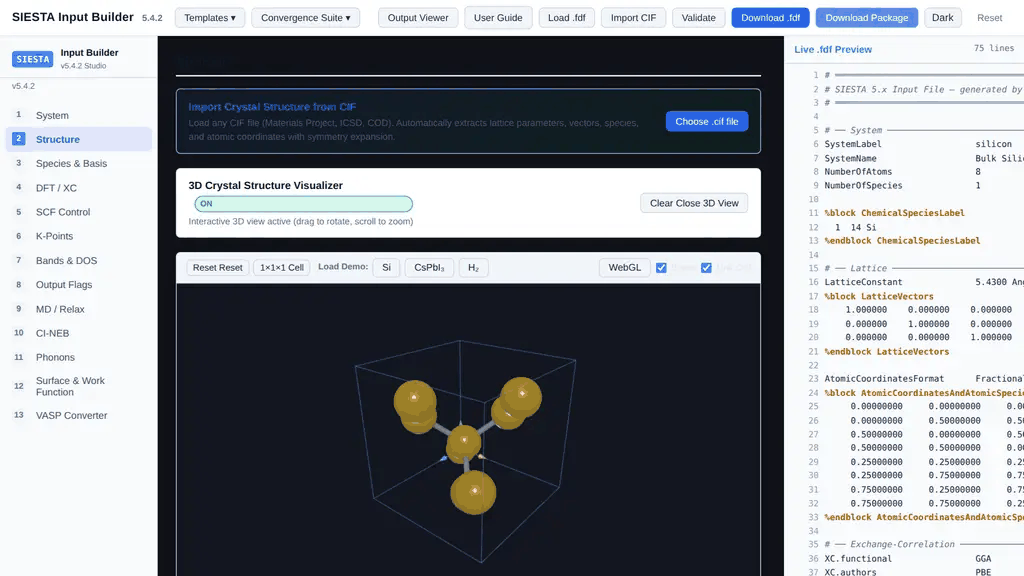
\includegraphics[width=0.92\textwidth]{figures/fig02_structure_3d.png}
\caption{Section 2 Structure interface: CIF import engine, slab vacuum padding/cleaving tools, atomic coordinates grid, and interactive 3D WebGL crystal viewer.}
\end{figure}


\subsection{Section 3 Species \& Basis: Pseudopotential Directory Scanner}

\subsubsection{The Remote Server Path Embedding Problem}
A frequent frustration in SIESTA calculations: you build an input on your laptop, copy the \texttt{.fdf} to a remote supercomputer cluster, and the job immediately crashes with:
\begin{verbatim}
Could not find pseudopotential file: Pb.psf
\end{verbatim}
In SIESTA, \texttt{\%block ChemicalSpeciesLabel} supports an optional fourth column specifying the absolute filesystem path to the pseudopotential file:
\begin{lstlisting}
%block ChemicalSpeciesLabel
  1   82  Pb   /path/to/pseudos/Pb.psf
  2   53  I    /path/to/pseudos/I.psf
%endblock ChemicalSpeciesLabel
\end{lstlisting}
When specified, SIESTA reads the pseudopotentials directly from that directory regardless of where you submit the job from!

\subsubsection{Folder Scanner \& Real-Time Matcher}
In **Step 1**, enter the absolute path where your pseudopotentials reside on the cluster (e.g., \texttt{/scratch/user/pseudos}).
In **Step 2**, click **Scan Folder** and choose the local folder on your computer:
\begin{itemize}[leftmargin=*]
 \item The browser uses HTML5 `webkitdirectory` to scan filenames locally without uploading file content.
 \item Click **Auto-Assign All**: The builder matches elements (e.g. symbol `Pb` matches `Pb.psf`, `Pb_pbe.psf`, or `Pb.psml`).
 \item \textbf{Status Badges:} The table displays green **`Found`** badges for confirmed files and amber **`Missing`** badges for missing pseudopotentials.
\end{itemize}

\subsubsection{Basis Set Customization}
\begin{itemize}[leftmargin=*]
 \item \textbf{\texttt{PAO.BasisSize}:} Select \texttt{DZP} for production calculations; \texttt{SZ} for quick initial geometry screening.
 \item \textbf{\texttt{PAO.EnergyShift}:} Slider and text box with unit conversion (meV, Ry, eV). Default is \texttt{100 meV}.
 \item \textbf{Soft Confinement Drawer:} Toggle \texttt{PAO.SoftDefault true} to soften orbital second derivatives at cutoff boundaries, suppressing eggbox oscillations.
\end{itemize}

\begin{figure}[h!]
\centering
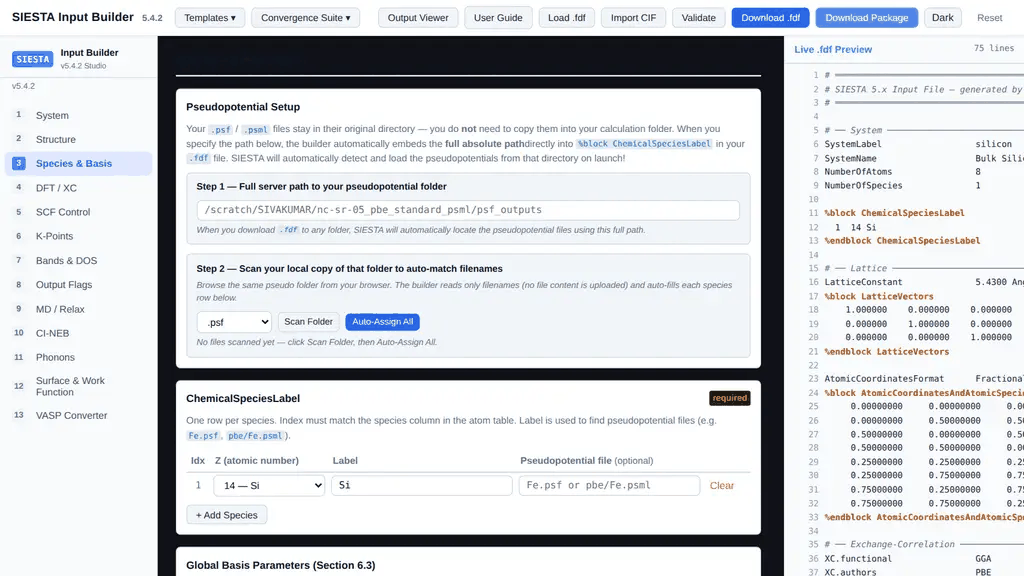
\includegraphics[width=0.92\textwidth]{figures/fig03_species_basis.png}
\caption{Section 3 Species \& Basis: Local folder scanner, automatic pseudopotential filename matching with real-time status badges, ChemicalSpeciesLabel table, and DZP basis parameters.}
\end{figure}
\subsection{Section 4 DFT / XC: Exchange-Correlation, vdW \& DFT+U}
\begin{itemize}[leftmargin=*]
 \item \textbf{XC Functional \& Authors:} Select functional type (GGA, LDA, VDW) and author parameterization (PBE, PBEsol, CA, revPBE).
 \item \textbf{\texttt{MeshCutoff}:} Energy cutoff governing real-space grid fineness. Standard values: 250–350 Ry for semiconductors; 350–450 Ry for oxides and transition metals.
 \item \textbf{Grimme DFT-D3 Dispersion:} Toggle \texttt{DFTD3 true} with choice of zero damping or Becke-Johnson (BJ) damping.
 \item \textbf{Spin Mode:} Toggle between \texttt{unpolarized}, \texttt{polarized} (collinear), \texttt{non-collinear}, and \texttt{spin-orbit}.
 \item \textbf{Magnetic State Assistant:} Click presets for Ferromagnetic (all spins aligned), Antiferromagnetic (alternating $\pm S$), or Non-collinear spiral spins to auto-format the \texttt{\%block DM.InitSpin} block.
 \item \textbf{DFT+U Assistant (\texttt{\%block DFTU.Proj}):} For transition metals ($Ni, Co, Fe, Ti$) or rare earths ($Ce$) where standard DFT fails due to self-interaction errors:
 \begin{itemize}
 \item Enable DFT+U and select species.
 \item Specify orbital shell ($d$ or $f$), Hubbard on-site Coulomb $U$ (eV), and Hund's exchange $J$ (eV).
 \item Automatically formats the formal SIESTA \texttt{\%block DFTU.Proj} block.
 \end{itemize}
\end{itemize}

\begin{figure}[h!]
\centering
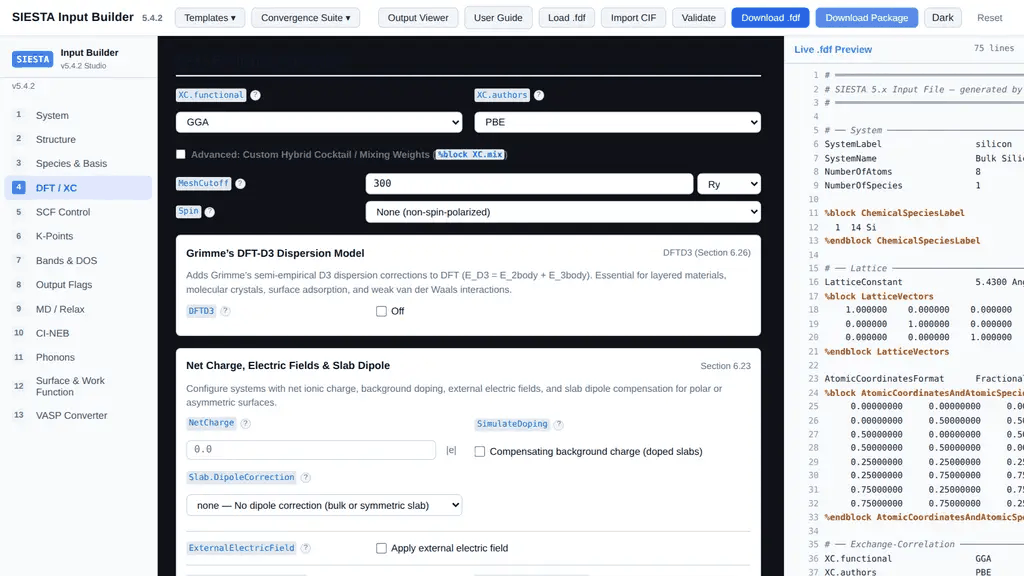
\includegraphics[width=0.92\textwidth]{figures/fig04_dft_xc.png}
\caption{Section 4 DFT / XC: Exchange-correlation functionals, MeshCutoff, Grimme DFT-D3 dispersion, spin-polarization modes, and on-site DFT+U assistant.}
\end{figure}
\subsection{Section 5 SCF Control: Convergence \& Mixing}
\begin{itemize}[leftmargin=*]
 \item \textbf{\texttt{MaxSCFIterations}:} Maximum iteration limit (typically 100–150).
 \item \textbf{\texttt{DM.Tolerance}:} Convergence density matrix threshold (typically \texttt{1.0d-4} to \texttt{1.0d-5}).
 \item \textbf{\texttt{DM.MixingWeight}:} Linear mixing parameter. \textbf{Hidden Troubleshooting Tip:} If your calculation diverges or oscillates with wild energy swings, reduce mixing weight from \texttt{0.25} down to \texttt{0.05} or \texttt{0.08}.
 \item \textbf{\texttt{DM.NumberPulay}:} Pulay DIIS history depth (typically 6 to 8).
 \item \textbf{\texttt{ElectronicTemperature}:} Fermi-Dirac smearing width (typically \texttt{25 meV} for metals; \texttt{0 meV} for insulators).
 \item \textbf{\texttt{DM.UseSaveDM}:} Toggle to \texttt{true} when restarting a calculation from an existing \texttt{SystemLabel.DM} density matrix file.
\end{itemize}

\subsection{Section 6 K-Points: Reciprocal Mesh \& High-Symmetry Band Path}

\subsubsection{Reciprocal Mesh Setup}
Configure Monkhorst-Pack grid divisions ($N_x \times N_y \times N_z$) and displacement shifts ($0.5$ for off-$\Gamma$, $0.0$ for $\Gamma$-centered).
\textbf{Dimensionality Protection:} If modeling a 2D slab or surface, the builder displays a guidance note reminding you to set $k_z = 1$.

\subsubsection{ Automated High-Symmetry Band Path Generator}
Located in the **High-Symmetry Band Path Generator** card:
\begin{itemize}[leftmargin=*]
 \item Click **Auto-Detect Lattice Path**: The builder inspects your lattice vectors and identifies the Bravais lattice type (Cubic, FCC, BCC, Tetragonal, Hexagonal, Rhombohedral, Slabs).
 \item It pre-populates standard crystallography paths (e.g. $\Gamma \to X \to W \to L \to \Gamma$ for FCC crystals; $\Gamma \to M \to K \to \Gamma$ for hexagonal/2D systems).
 \item Customize division points per line segment and click **Apply to BandLines**.
 \item \textbf{Fatbands Export:} Toggle \texttt{WFS.Write.For.Bands true} to output wavefunctions into \texttt{SystemLabel.fullBZ.WFSX} for orbital-projected band structure analysis.
\end{itemize}

\begin{figure}[h!]
\centering
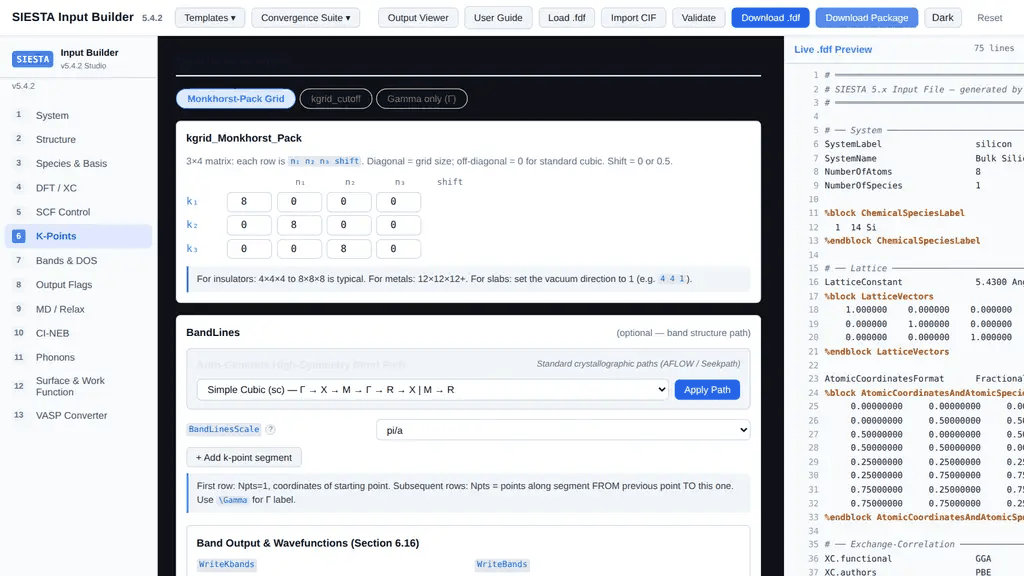
\includegraphics[width=0.92\textwidth]{figures/fig05_kpoints.png}
\caption{Section 6 K-Points: Monkhorst-Pack grid inputs and the automated High-Symmetry Band Path Generator pre-populating standard AFLOW/Seekpath crystallographic paths.}
\end{figure}


\subsection{Section 7 Bands \& DOS / PDOS: Electronic Structure}
\begin{itemize}[leftmargin=*]
 \item \textbf{Projected DOS (\texttt{\%block ProjectedDensityOfStates}):} Configure energy window ($E_{\text{min}}$ to $E_{\text{max}}$), Gaussian peak broadening width ($\sigma$), number of points, and energy units. Toggle \texttt{EF} to align energy relative to the Fermi level.
 \item \textbf{Custom PDOS k-grid:} Toggle \texttt{PDOS.kgrid.MonkhorstPack} to use a denser $k$-point mesh for the DOS calculation than was used for the self-consistent SCF charge density.
 \item \textbf{Local Density of States (LDOS):} Spatial energy window slice (\texttt{\%block LocalDensityOfStates}).
    \item \textbf{\texttt{WriteEigenvalues}:} Toggle to write all Kohn-Sham eigenvalues to \texttt{SystemLabel.EIG}.
    \item \textbf{3D Molecular Orbital \& HOMO / LUMO Visualizer (\texttt{.cube}):} Upload any 3D Gaussian Cube file from SIESTA (\texttt{denchar}, \texttt{grid2cube}), Quantum ESPRESSO (\texttt{pp.x}), ORCA, or Gaussian. The visualizer executes real-time Marching Cubes isosurface extraction in WebGL, displaying dual-phase lobes ($+\psi$ in cyan, $-\psi$ in amber), interactive isovalue threshold sliders, transparency controls, CPK molecular framework (atoms and covalent bonds), and high-resolution PNG snapshot capture.
\end{itemize}

\begin{figure}[h!]
\centering
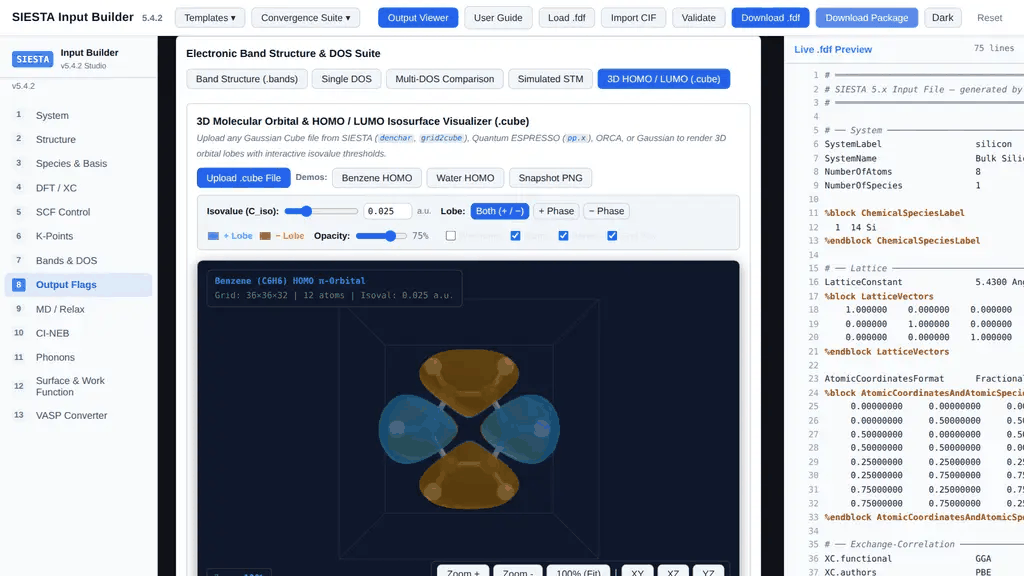
\includegraphics[width=0.92\textwidth]{figures/fig11_homo_lumo_3d.png}
\caption{Section 7 \& Section 8: Interactive 3D Molecular Orbital and HOMO / LUMO Isosurface Visualizer showing Benzene $C_6H_6$ $\pi$-orbital lobes, isovalue slider, phase selectors, and CPK molecular framework.}
\end{figure}
\subsection{Section 8 Output Flags \& Results Viewer}
This section contains two distinct workspaces selected via top tab pills:

\subsubsection{Tab 1: FDF Output Flags}
Configure which files SIESTA produces:
\begin{itemize}[leftmargin=*]
 \item \textbf{Trajectories:} \texttt{WriteMDXmol true} ($\implies$ \texttt{.ANI} for VMD/JMol/OVITO), \texttt{WriteMDhistory true} ($\implies$ \texttt{.MDE} thermodynamic record), \texttt{WriteCoorXmol true} ($\implies$ \texttt{.xyz}).
 \item \textbf{Real-Space Grids:} \texttt{SaveRho} (charge density), \texttt{SaveDeltaRho} (charge difference), \texttt{SaveElectrostaticPotential} ($\implies$ \texttt{.VH} for work functions), \texttt{SaveTotalPotential} (\texttt{.VT}), \texttt{SaveHS} (\texttt{.HSX} matrices).
 \item \textbf{Section 6.29 Accounting Flags:} \texttt{AllocReportLevel} (0 to 4 in \texttt{.alloc}), \texttt{TimerReportThreshold}, \texttt{UseParallelTimer}, \texttt{MaxWalltime} queue limit, and \texttt{MaxWalltime.Slack}.
\end{itemize}

\subsubsection{Tab 2: Results Analysis \& Viewer Workspace}
Drag and drop (or upload) calculation output files:
\begin{itemize}[leftmargin=*]
 \item \textbf{Log Inspector (\texttt{.out}):} Extracts final total energy, Fermi energy, mesh cutoff used, cell volume, forces, and normal completion status.
 \item \textbf{Convergence Charts (\texttt{.MDE} / \texttt{.out}):} Interactive SVG curves showing total energy convergence across geometry steps and SCF density matrix residual history.
 \item \textbf{3D Trajectory Player (\texttt{.ANI}):} Play molecular dynamics or relaxation movies. Scrub through frames with a slider, control playback speed, step forward/backward, and toggle between WebGL and Canvas 2D rendering.
 \item \textbf{Electronic Band Structure Plotter (\texttt{.bands}):} Renders $E(\mathbf{k})$ dispersion with adjustable Fermi level offset, high-symmetry tick labels, and PNG/SVG export.
 \item \textbf{DOS Plotter Suite (\texttt{.EIG} / \texttt{.PDOS.xml}):} Calculates Total DOS using the official `Util/Eig2DOS` algorithm with Gaussian or Lorentzian broadening, decomposes orbital projections ($s, p, d, f$), and exports data columns.
 \item \textbf{Simulated STM Topography:} Renders constant-height and constant-current STM topography maps based on the Tersoff-Hamann approximation.
 \item \textbf{TIMES Execution Profiler:} Upload your \texttt{SystemLabel.times} or \texttt{TIMES} file. Displays total elapsed wall-clock time, cumulative core CPU hours, MPI node count, load balancing ratio ($Avg/Max$), top routine bottleneck bar charts, and a searchable, sortable routine table with 1-click clipboard copy!
\end{itemize}

\begin{figure}[h!]
\centering
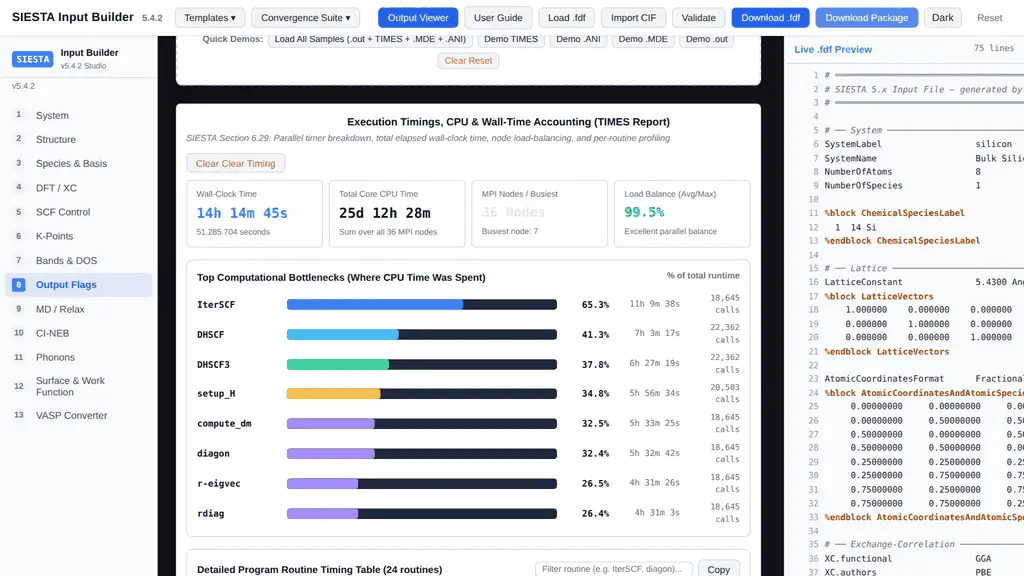
\includegraphics[width=0.92\textwidth]{figures/fig06_output_times.png}
\caption{Section 8 Output Flags \& Results Viewer: Section 6.29 parallel execution timer breakdown (wall-clock time, core CPU hours, node load-balancing ratio, and routine bottleneck chart).}
\end{figure}


\subsection{Section 9 MD / Relaxation: Geometry Optimization \& Dynamics}
\begin{itemize}[leftmargin=*]
 \item \textbf{Optimizers:} Select \texttt{CG} (standard conjugate gradient), \texttt{Broyden}, or \texttt{FIRE} (superior for complex structures far from equilibrium).
 \item \textbf{Tolerances:} Set maximum atomic force component (\texttt{MD.MaxForceTol}, e.g. \texttt{0.04 eV/\AA}) and maximum stress component (\texttt{MD.MaxStressTol}, e.g. \texttt{1.0 GPa}).
 \item \textbf{Cell Relaxation:} Toggle \texttt{MD.VariableCell true} to relax cell vectors, or activate \texttt{Constant.Volume} to relax cell shape while keeping total volume fixed.
 \item \textbf{Restarting Relaxations:} Check \texttt{MD.UseSaveCG true} to resume conjugate-gradient history from \texttt{SystemLabel.CG}.
 \item \textbf{Molecular Dynamics Ensembles:} Toggle \texttt{Verlet} (microcanonical $NVE$), \texttt{Nose} (canonical $NVT$ thermostat), or \texttt{ParrinelloRahman} (isobaric-isothermal $NPT$). Set time step (\texttt{MD.LengthTimeStep}, e.g. \texttt{1.0 fs}) and temperatures.
\end{itemize}

\subsection{Section 10 CI-NEB Suite: Transition State Search}
\begin{itemize}[leftmargin=*]
 \item \textbf{Climbing Image NEB:} Identifies minimum energy pathways (MEP) and saddle-point transition states for chemical reactions, vacancy diffusion, and ion migration.
 \item \textbf{IDPP Interpolation:} Upload Initial and Final state CIF or FDF files. The builder uses Image Dependent Pair Potential (IDPP) interpolation to generate $N$ smooth, unskewed intermediate reaction frames without atom collisions.
 \item \textbf{3D Reaction Pathway Slider:} Scrub through images to inspect the reaction path in 3D.
 \item \textbf{Integrated Pseudopotential Verification:} Confirms that all reacting elements have valid pseudopotential files available.
 \item \textbf{1-Click Download CI-NEB Suite (.zip):} Generates all image FDF files (\texttt{image\_00.fdf} to \texttt{image\_0N.fdf}), automated ASE CI-NEB driver (\texttt{cineb\_siesta\_driver.py}), barrier plotter (\texttt{plot\_neb\_barrier.py}), and parallel SLURM runner (\texttt{run\_cineb.sh}).
\end{itemize}

\begin{figure}[h!]
\centering
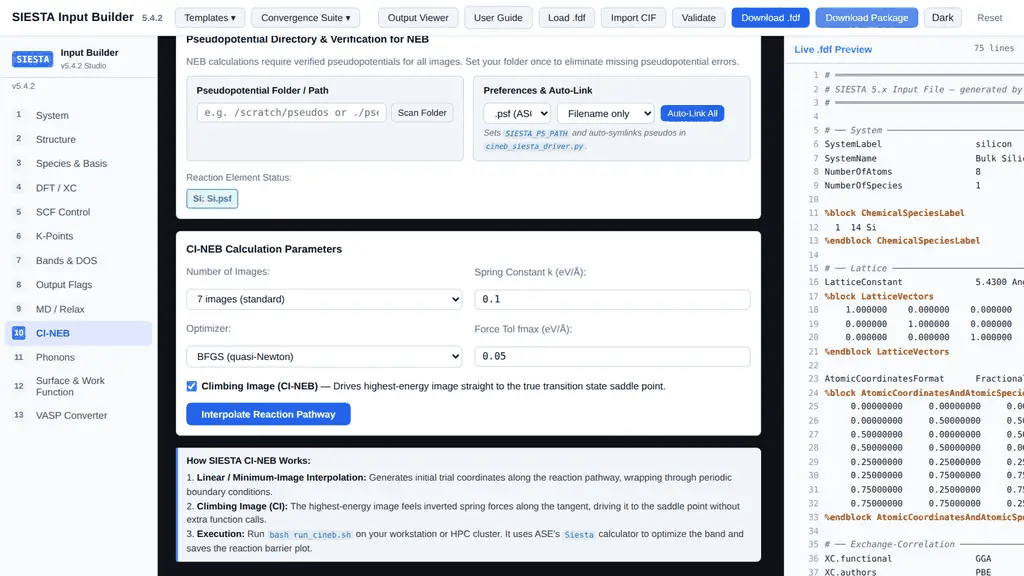
\includegraphics[width=0.92\textwidth]{figures/fig07_cineb.png}
\caption{Section 10 CI-NEB Suite: Reaction transition state search, IDPP pair-potential interpolation, 3D pathway slider, and 1-click CI-NEB package generator.}
\end{figure}


\subsection{Section 11 Phonons \& Vibrations: Force Constants \& Vibra}
\begin{itemize}[leftmargin=*]
 \item \textbf{Finite Displacement Method:} Calculates harmonic force constants by displacing atoms in small finite steps (\texttt{MD.TypeOfRun FC}).
 \item \textbf{Displacement Amplitude:} \texttt{FC.Displacement} (default \texttt{0.04 Bohr} $\approx 0.021\text{ \AA}$).
 \item \textbf{Atom Subsets:} Select subset of atoms to displace (\texttt{FC.first} and \texttt{FC.last}) to focus on surface adsorbate vibrations while omitting substrate atoms.
 \item \textbf{Polar Materials \& LO-TO Splitting:} Toggle \texttt{BornCharge true} to compute Born effective charge tensors and macroscopic dielectric matrices.
 \item \textbf{Supercell Builder:} Expands the unit cell into a $2\times2\times2$ supercell to account for interatomic force ranges beyond the primary cell.
 \item \textbf{1-Click Download Phonon Suite (.zip):} Generates \texttt{supercell\_fc.fdf}, \texttt{vibra.fdf}, \texttt{plot\_phonon\_dispersion.py}, and \texttt{run\_phonon.sh}.
\end{itemize}

\begin{figure}[h!]
\centering
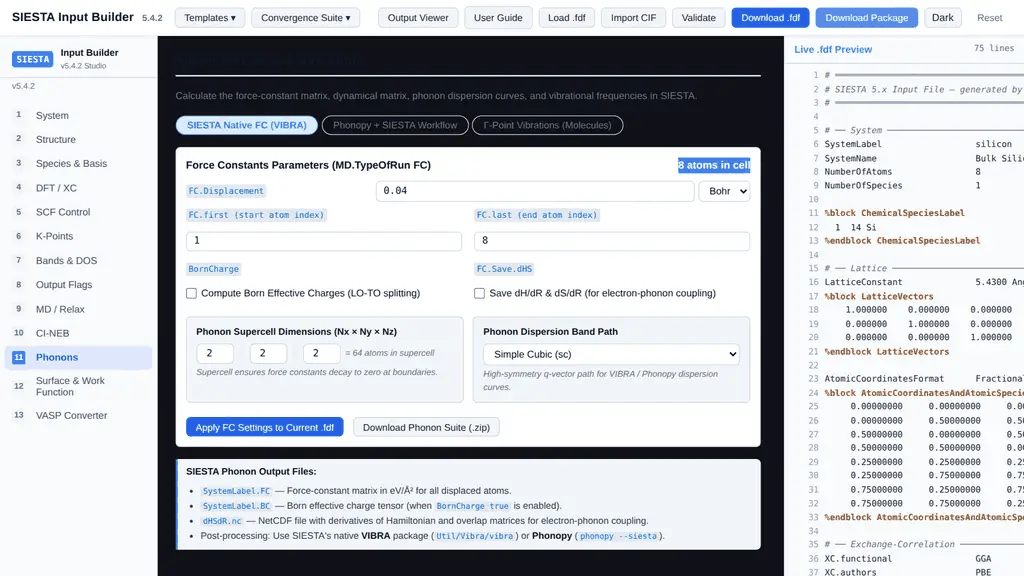
\includegraphics[width=0.92\textwidth]{figures/fig08_phonons.png}
\caption{Section 11 Phonons: Finite displacement force constants calculation (MD.TypeOfRun FC), supercell builder, Born effective charges, and Vibra suite export.}
\end{figure}


\subsection{Section 12 Surface, Work Function \& Adsorption Analysis}
A dedicated post-DFT surface science laboratory containing 5 specialized tools:
\begin{enumerate}[leftmargin=*]
 \item \textbf{Adsorption Energy ($E_{\text{ads}}$) Calculator:} Input total energy of the complex, clean slab, and isolated molecule to calculate binding strength:
 \begin{equation}
 E_{\text{ads}} = E_{\text{total}} - E_{\text{slab}} - E_{\text{mol}}
 \end{equation}
 Categorizes interaction as physical physisorption ($|E_{\text{ads}}| < 0.8\text{ eV}$) or chemical bonding ($|E_{\text{ads}}| > 1.0\text{ eV}$).
 \item \textbf{Planar Average Charge Density Difference (CDD):} Upload difference cube or data file. Displays real-space charge redistribution $\Delta\bar{\rho}(z)$, electron accumulation zones (bonding), depletion zones (charge loss), and cumulative charge transfer $\Delta Q(z)$ with interface dipole $\mu$ in Debye.
 \item \textbf{Multi-Surface Work Function Comparison Studio:} Compare multiple surface states (e.g. clean perovskite vs passivated perovskite). Automatically aligns Fermi levels, extracts asymptotic vacuum plateaus $V_{\text{vac}}$, computes work functions ($\Phi = V_{\text{vac}} - E_F$), evaluates dipole steps ($\Delta V$), and exports vector SVG, 300 DPI PNG, 300 DPI TIFF, or raw column data.
 \item \textbf{3D Energy Band Alignment & Heterojunction Diagram:} Construct publication-ready band alignment diagrams for solar cells, LEDs, and catalysts. Add custom layers (absorber, ETL, HTL, metal contacts), adjust CBM/VBM levels, toggle curved carrier extraction arrows ($e^-$ and $h^+$), and choose 3D perspective shading.
 \item \textbf{SIESTA Grid Workflow Drawer:} Provides verified terminal commands for Util/Macroave (\texttt{macroave < macroave.in}) and Util/Grid (\texttt{grid2cube SystemLabel.VH}).
\end{enumerate}

\begin{figure}[h!]
\centering
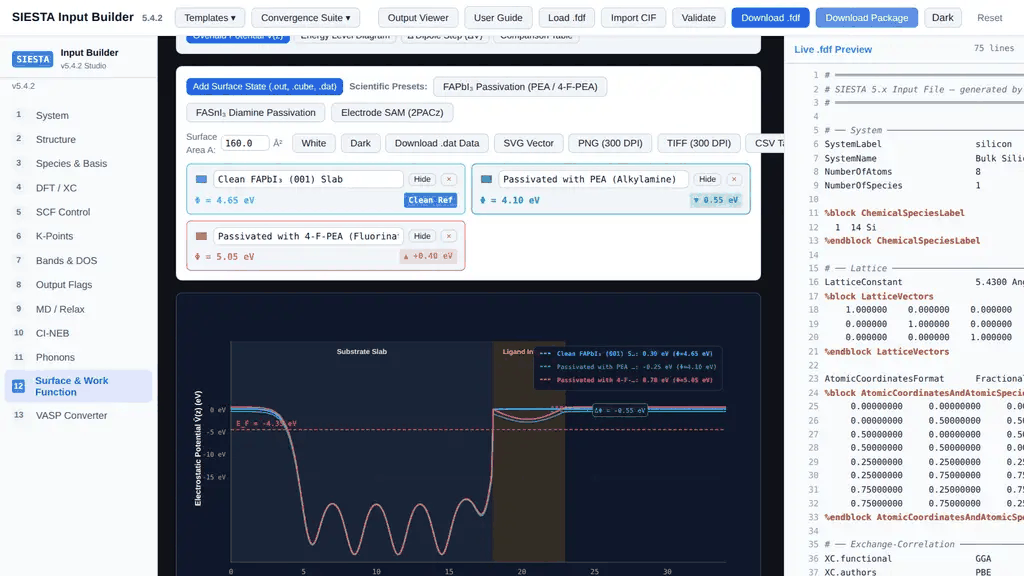
\includegraphics[width=0.92\textwidth]{figures/fig09_workfunction.png}
\caption{Section 12 Surface \& Work Function Studio: Overlaid planar average potential profiles V̄(z), flat asymptotic vacuum plateaus, work function reduction ΔΦ, and surface dipole calculation.}
\end{figure}


\subsection{Section 13 VASP to FDF Converter (ASE GUI Constraints)}
Designed specifically for researchers who set up geometry constraints in ASE GUI and save as VASP POSCAR:
\begin{itemize}[leftmargin=*]
 \item \textbf{Side-by-Side Dual-Pane Interface:} Paste or upload a VASP \texttt{POSCAR} or \texttt{CONTCAR} file on the left; view the live generated SIESTA \texttt{.fdf} on the right.
 \item \textbf{ASE GUI Selective Dynamics Parser:} Automatically parses \texttt{Selective dynamics} and flags:
 \begin{itemize}
 \item \texttt{F F F}: Fully fixed in all directions $\implies$ serialized as \texttt{atom [1 -- 4]}.
 \item \texttt{T T F}: Fixed along $z$ only $\implies$ serialized with trailing dot real notation: \texttt{atom i 0. 0. 1.} (allows in-plane $xy$ relaxation while preventing out-of-plane buckling).
 \item \texttt{F F T}: Fixed in $xy$ plane only $\implies$ serialized as \texttt{atom i 1. 1. 0.}.
 \item \texttt{T T T}: Completely free to relax.
 \end{itemize}
 \item \textbf{SIESTA Section 7.7 Controls:}
 \begin{itemize}
 \item Syntax selector: \texttt{atom [1 -- 4]} (modern bracket notation), \texttt{atom from 1 to 4}, or explicit list \texttt{atom 1 2 3 4}.
 \item Cell vector locks: Checkbox for \texttt{cell-vector C} to freeze the vacuum axis during relaxation.
 \item Stress tensor locks: Checkboxes for \texttt{stress XX}, \texttt{YY}, \texttt{ZZ}, \texttt{XY}.
 \item Element locks: Checkboxes to freeze all atoms of a species by atomic number (e.g. \texttt{Z 82} for Pb).
 \end{itemize}
 \item \textbf{Direct PP Folder Field:} Enter pseudopotential directory path directly in the converter ribbon.
 \item \textbf{Load to Workspace Button:} Clicking this transfers the converted crystal coordinates, lattice vectors, chemical species, and pseudopotential paths into Section 2 and the 3D visualizer!
\end{itemize}

\begin{figure}[h!]
\centering
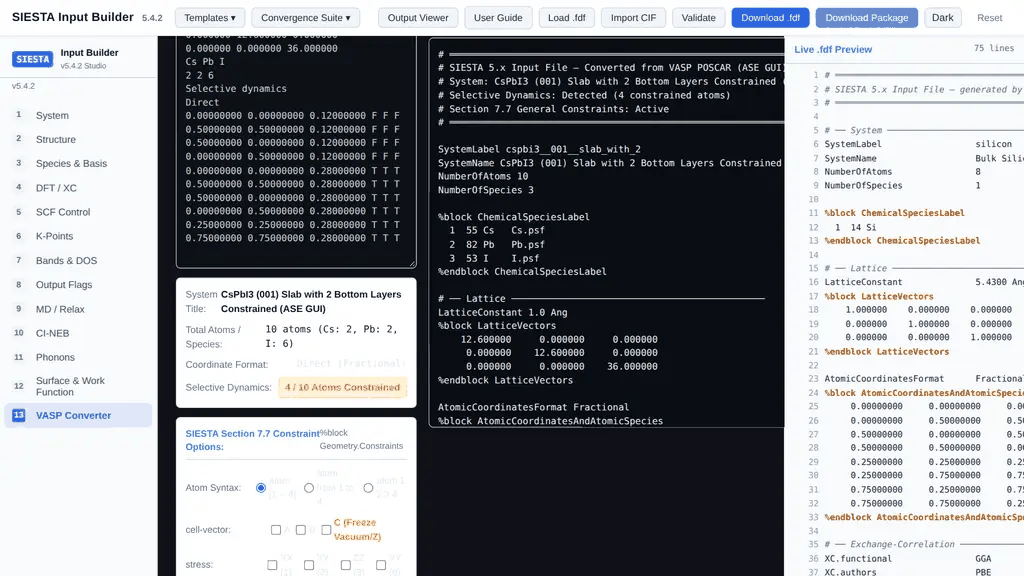
\includegraphics[width=0.92\textwidth]{figures/fig10_vasp_converter.png}
\caption{Section 13 VASP to FDF Converter: Side-by-side dual-pane workspace, ASE GUI Selective Dynamics parsing, Section 7.7 General Constraints controls, and 1-click Load to Workspace.}
\end{figure}

\subsection{Section 14 Charge Transfer \& Real-Space Grid Densities Analysis (Section 6.24)}
SIESTA evaluates electron charge densities, deformation densities, and electrostatic potentials directly on the real-space mesh used by DHSCF. Section 14 provides a comprehensive suite to configure mesh output and analyze charge transfer:
\begin{itemize}[leftmargin=*]
    \item \textbf{Charge Densities on Mesh:} Toggles for \texttt{SaveRho} ($\rho(\mathbf{r})$ valence density in \texttt{.RHO}), \texttt{SaveDeltaRho} ($\delta\rho(\mathbf{r}) = \rho(\mathbf{r}) - \rho_{\text{atm}}(\mathbf{r})$ deformation density in \texttt{.DRHO}), \texttt{SaveRhoXC} (valence density + core corrections for XC energy in \texttt{.RHOXC}), \texttt{SaveIonicCharge} (soft diffuse ionic charge in \texttt{.IOCH}), and \texttt{SaveTotalCharge} (\texttt{.TOCH}).
    \item \textbf{Electrostatic \& Effective Potentials:} Toggles for \texttt{SaveElectrostaticPotential} ($V_H + V_{\text{local}}$ in \texttt{.VH}), \texttt{SaveTotalPotential} ($V_H + V_{\text{xc}} + V_{\text{local}}$ in \texttt{.VT}), and \texttt{SaveNeutralAtomPotential} (\texttt{.VNA}). Enabling \texttt{SaveTotalPotential} automatically triggers the output of the vacuum level in stdout for work function calculations.
    \item \textbf{Henkelman Bader Analysis Options:} Toggles \texttt{SaveBaderCharge} to add generalized Gaussian model core charges to the valence density (\texttt{.BADER}), configurable via \texttt{bader-core-radius-standard} (default 1.3~Bohr) and \texttt{bader-core-radius-hydrogen} (default 0.4~Bohr).
    \item \textbf{Bader Charge Transfer Studio (\texttt{ACF.dat}):} Upload or paste Henkelman Bader output to compute net charge transfer $\Delta Q_i = Z_{\text{val}, i} - Q_{\text{Bader}, i}$ per atom and species, total electron conservation, and interfacial dipole moment $\mu_z$ (in Debye and $e\cdot\text{\AA}$).
    \item \textbf{Planar Average Charge Displacement $\Delta\bar{\rho}(z)$ \& $\Delta Q(z)$:} Dual-axis interactive SVG chart displaying planar average charge redistribution and cumulative transferred charge $\Delta Q(z) = \int \Delta\bar{\rho}(z') \, dz'$ across interfaces and slabs.
    \item \textbf{3D Charge Difference $\Delta\rho(\mathbf{r})$ Viewer:} Interactive Dual-Engine (WebGL + 2D Canvas) 3D isosurface viewer rendering charge accumulation ($+\delta\rho$, cyan) and depletion ($-\delta\rho$, amber) lobes.
\end{itemize}

\begin{figure}[h!]
\centering
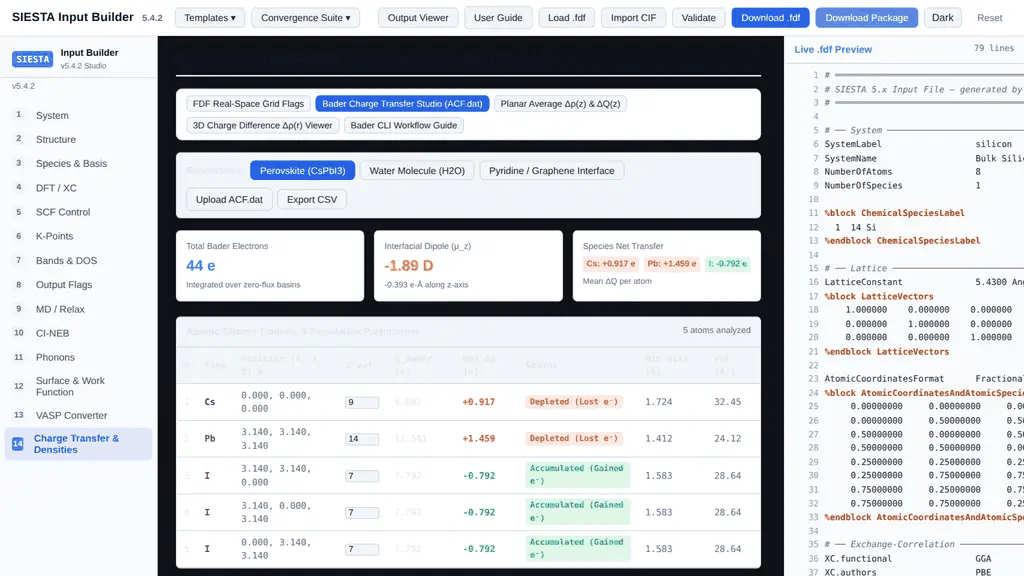
\includegraphics[width=0.92\textwidth]{figures/fig12_chargetransfer.png}
\caption{Section 14 Charge Transfer Analysis: Bader Charge Transfer Studio (ACF.dat), per-atom net $\Delta Q$ partitioning, interfacial dipole moment, and 1-click Section 6.24 real-space grid presets.}
\end{figure}

\subsection{The Live .fdf Preview Pane}
\begin{itemize}[leftmargin=*]
 \item Real-time bi-directional reflection: Every input field, checkbox, slider, or table edit re-serializes the FDF instantly.
 \item Syntax color coding: Comments (\texttt{\# ...}) appear in muted gray italic; data block delimiters (\texttt{\%block} / \texttt{\%endblock}) appear in bold amber; keywords appear in high-contrast text.
 \item Line number counter in the header indicates the total length of the generated file.
\end{itemize}

\newpage
% ── SECTION 4 ───────────────────────────────────────────────────────────────
\section{Step-by-Step Practical Tutorials}

\subsection{Tutorial A: Bulk Silicon Optimization \& Band Structure}
\begin{enumerate}[leftmargin=*]
 \item Click **Templates ▾** in the top toolbar and select **Bulk SCF (single-point)**.
 \item Set \texttt{SystemLabel} to \texttt{silicon\_bulk} in Section 1.
 \item In Section 3, click **Scan Folder** to match \texttt{Si.psf} or \texttt{Si.psml}.
 \item In Section 6, click **Auto-Detect Lattice Path** to populate the FCC path: $\Gamma \to X \to W \to L \to \Gamma$.
 \item In Section 9, select optimizer \texttt{CG} and set \texttt{MD.MaxForceTol 0.02 eV/Ang}.
 \item Click **Download Package** in the toolbar.
 \item On your cluster, extract the package and submit:
\begin{lstlisting}[language=bash]
unzip silicon_bulk.zip && cd silicon_bulk
bash run_siesta.sh
\end{lstlisting}
 \item After completion, open Section 8 Tab 2, drag and drop \texttt{silicon\_bulk.bands}, and inspect the electronic dispersion curves!
\end{enumerate}

\subsection{Tutorial B: $FAPbI_3$ Perovskite Slab with Fixed Substrate}
\begin{enumerate}[leftmargin=*]
 \item In the top toolbar, click **Import CIF** and select \texttt{FAPbI3\_cubic.cif}.
 \item In Section 2, locate the ** Slab \& Vacuum Tools** card. Set vacuum thickness to \texttt{20.0 \AA} and click **Add Vacuum**. Click **Center Slab in Cell**.
 \item Open Section 13 **VASP to FDF Converter** if importing an ASE GUI relaxed geometry, or freeze bottom layers ($z < 15\text{ \AA}$) via the Section 7.7 constraint controls. Check \texttt{cell-vector C} to ensure the vacuum gap remains constant.
 \item In Section 4, ensure \texttt{Slab.DipoleCorrection true} and \texttt{DFTD3 true} are enabled. Set \texttt{MeshCutoff 350 Ry}.
 \item In Section 6, verify the $k$-grid is set to $4 \times 4 \times 1$.
 \item In Section 8, enable \texttt{SaveElectrostaticPotential true} and \texttt{WriteMDXmol true}.
 \item Click **Download .fdf**.
 \item Upon calculation completion, drag and drop \texttt{FAPbI3\_slab.ANI} into Section 8 to play the relaxation movie in 3D!
 \item Run \texttt{grid2cube FAPbI3\_slab.VH} and upload \texttt{FAPbI3\_slab.cube} into Section 12 to extract the vacuum plateau and calculate the work function: $\Phi = V_{\text{vac}} - E_F$.
\end{enumerate}

\newpage
% ── SECTION 5 ───────────────────────────────────────────────────────────────
\section{Troubleshooting, Edge Cases \& Power-User Tips}

\begin{table}[h]
\centering
\small
\begin{tabular}{p{4.2cm} p{5.5cm} p{6.8cm}}
\toprule
\textbf{Symptom / Error} & \textbf{Physical / Numerical Root Cause} & \textbf{Immediate GUI Remedy} \\
\midrule
\texttt{SCF does not converge} (energy oscillates wildly) & Charge sloshing between localized orbitals or metallic surface states & Go to Section 5: Lower \texttt{DM.MixingWeight} from 0.25 to 0.05. Increase \texttt{ElectronicTemperature} to 25–50 meV. \\
\addlinespace
\texttt{Could not find pseudopotential} & Missing `.psf`/`.psml` file or incorrect path on remote cluster & In Section 3, specify the exact cluster folder in Step 1. The builder embeds the full path into \texttt{\%block ChemicalSpeciesLabel}. \\
\addlinespace
\texttt{Vacuum collapsing during relaxation} & \texttt{MD.VariableCell true} was enabled without locking the $c$-axis & In Section 13 or 9, activate \texttt{cell-vector C} in \texttt{\%block Geometry.Constraints} so only in-plane $a, b$ relax. \\
\addlinespace
\texttt{Eggbox ripple in forces} & Discrete real-space grid spacing is too coarse relative to core states & In Section 4, increase \texttt{MeshCutoff} to $\ge 350\text{ Ry}$. In Section 3, enable \texttt{PAO.SoftDefault true}. \\
\addlinespace
\texttt{Calculation runs out of wall time} & Long relaxation or molecular dynamics killed mid-step by SLURM & In Section 8, set \texttt{MaxWalltime} (e.g. \texttt{23.5 hours}) and \texttt{MaxWalltime.Slack 60 s} for a clean emergency restart. \\
\addlinespace
\texttt{Ghost dipole electric field in vacuum} & Asymmetric slab with polar adsorbate induced periodic image field & In Section 4, enable \texttt{Slab.DipoleCorrection true} and set direction to \texttt{z}. \\
\bottomrule
\end{tabular}
\caption{Comprehensive diagnostic matrix and troubleshooting remedies for SIESTA calculations.}
\end{table}

\subsection{Keyboard Shortcuts and Hidden Productivity Tips}
\begin{itemize}[leftmargin=*]
 \item \textbf{Tab-Separated Paste in Atom Table:} Highlight any cell in the atomic coordinates grid in Section 2 and press \textbf{Ctrl+V} to paste multi-column data directly from VESTA or text editors.
 \item \textbf{Camera Projection Snapping:} In the 3D Crystal Viewer, press the camera projection buttons to jump directly to primary axes ($X, Y, Z$).
 \item \textbf{1-Click Table Copy in TIMES Analyzer:} In Section 8 Tab 2, clicking **Copy** on the execution timer table copies formatted routine timings directly to your clipboard for pasting into reports or spreadsheets.
 \item \textbf{Direct Workspace Transfer:} In Section 13 (VASP Converter), clicking **Load to Workspace** converts your POSCAR structure, parses selective dynamics into Section 7.7 constraints, and injects the geometry directly into Section 2 and the 3D viewer without requiring manual file exports!
\end{itemize}

\vspace{1cm}
\begin{center}
\rule{0.6\textwidth}{0.8pt}\\[0.3cm]
\small \textbf{SIESTA Input Builder Web Studio — Documentation Version 5.4.2}\\[0.1cm]
\footnotesize Maintained by the Open-Source Materials Science Consortium
\end{center}

\end{document}
